%%%%%%%%%%%%%%%%%%%%%%%%%%%%%%%%%%%%%%%%%
% Beamer Presentation
% LaTeX Template
% Version 1.0 (10/11/12)
%
% This template has been downloaded from:
% http://www.LaTeXTemplates.com
%
% License:
% CC BY-NC-SA 3.0 (http://creativecommons.org/licenses/by-nc-sa/3.0/)
%
%%%%%%%%%%%%%%%%%%%%%%%%%%%%%%%%%%%%%%%%%

%----------------------------------------------------------------------------------------
%	PACKAGES AND THEMES
%----------------------------------------------------------------------------------------

\documentclass{beamer}

\mode<presentation> {

% The Beamer class comes with a number of default slide themes
% which change the colors and layouts of slides. Below this is a list
% of all the themes, uncomment each in turn to see what they look like.

%\usetheme{default}
%\usetheme{AnnArbor}
%\usetheme{Antibes}
%\usetheme{Bergen}
%\usetheme{Berkeley}
%\usetheme{Berlin}
%\usetheme{Boadilla}
%\usetheme{CambridgeUS}
%\usetheme{Copenhagen}
%\usetheme{Darmstadt}
%\usetheme{Dresden}
%\usetheme{Frankfurt}
%\usetheme{Goettingen}
%\usetheme{Hannover}
%\usetheme{Ilmenau}
%\usetheme{JuanLesPins}
%\usetheme{Luebeck}
\usetheme{Madrid}
%\usetheme{Malmoe}
%\usetheme{Marburg}
%\usetheme{Montpellier}
%\usetheme{PaloAlto}
%\usetheme{Pittsburgh}
%\usetheme{Rochester}
%\usetheme{Singapore}
%\usetheme{Szeged}
%\usetheme{Warsaw}

% As well as themes, the Beamer class has a number of color themes
% for any slide theme. Uncomment each of these in turn to see how it
% changes the colors of your current slide theme.

%\usecolortheme{albatross}
%\usecolortheme{beaver}
%\usecolortheme{beetle}
%\usecolortheme{crane}
%\usecolortheme{dolphin}
%\usecolortheme{dove}
%\usecolortheme{fly}
%\usecolortheme{lily}
%\usecolortheme{orchid}
%\usecolortheme{rose}
%\usecolortheme{seagull}
%\usecolortheme{seahorse}
\usecolortheme{whale}
%\usecolortheme{wolverine}

%\setbeamertemplate{footline} % To remove the footer line in all slides uncomment this line
%\setbeamertemplate{footline}[page number] % To replace the footer line in all slides with a simple slide count uncomment this line

%\setbeamertemplate{navigation symbols}{} % To remove the navigation symbols from the bottom of all slides uncomment this line
}

\usepackage{graphicx} % Allows including images
\usepackage{booktabs} % Allows the use of \toprule, \midrule and \bottomrule in tables
\usepackage[utf8]{inputenc}
\usepackage[russian]{babel}
\usepackage{hyperref}
\usepackage{ulem}
\usepackage{amsmath}
\usepackage{algorithm}
\usepackage{algpseudocode}

\newcommand{\angstrom}{\textup{\AA}}
\newcommand{\eps}{\varepsilon}
\newcommand{\la}{\leftarrow}
%----------------------------------------------------------------------------------------
%	TITLE PAGE
%----------------------------------------------------------------------------------------

\title{Разработка среды для построения структур белковых алгоритмов} % The short title appears at the bottom of every slide, the full title is only on the title page

\author{Рак Алексей} % Your name
\date{\today} % Date, can be changed to a custom date

\begin{document}

\begin{frame}
\titlepage % Print the title page as the first slide
\end{frame}

\begin{frame}
\frametitle{План} % Table of contents slide, comment this block out to remove it
\tableofcontents % Throughout your presentation, if you choose to use \section{} and \subsection{} commands, these will automatically be printed on this slide as an overview of your presentation
\end{frame}

%----------------------------------------------------------------------------------------
%	PRESENTATION SLIDES
%----------------------------------------------------------------------------------------
\section{ Среда}
\begin{frame}
\frametitle{PyMOL}
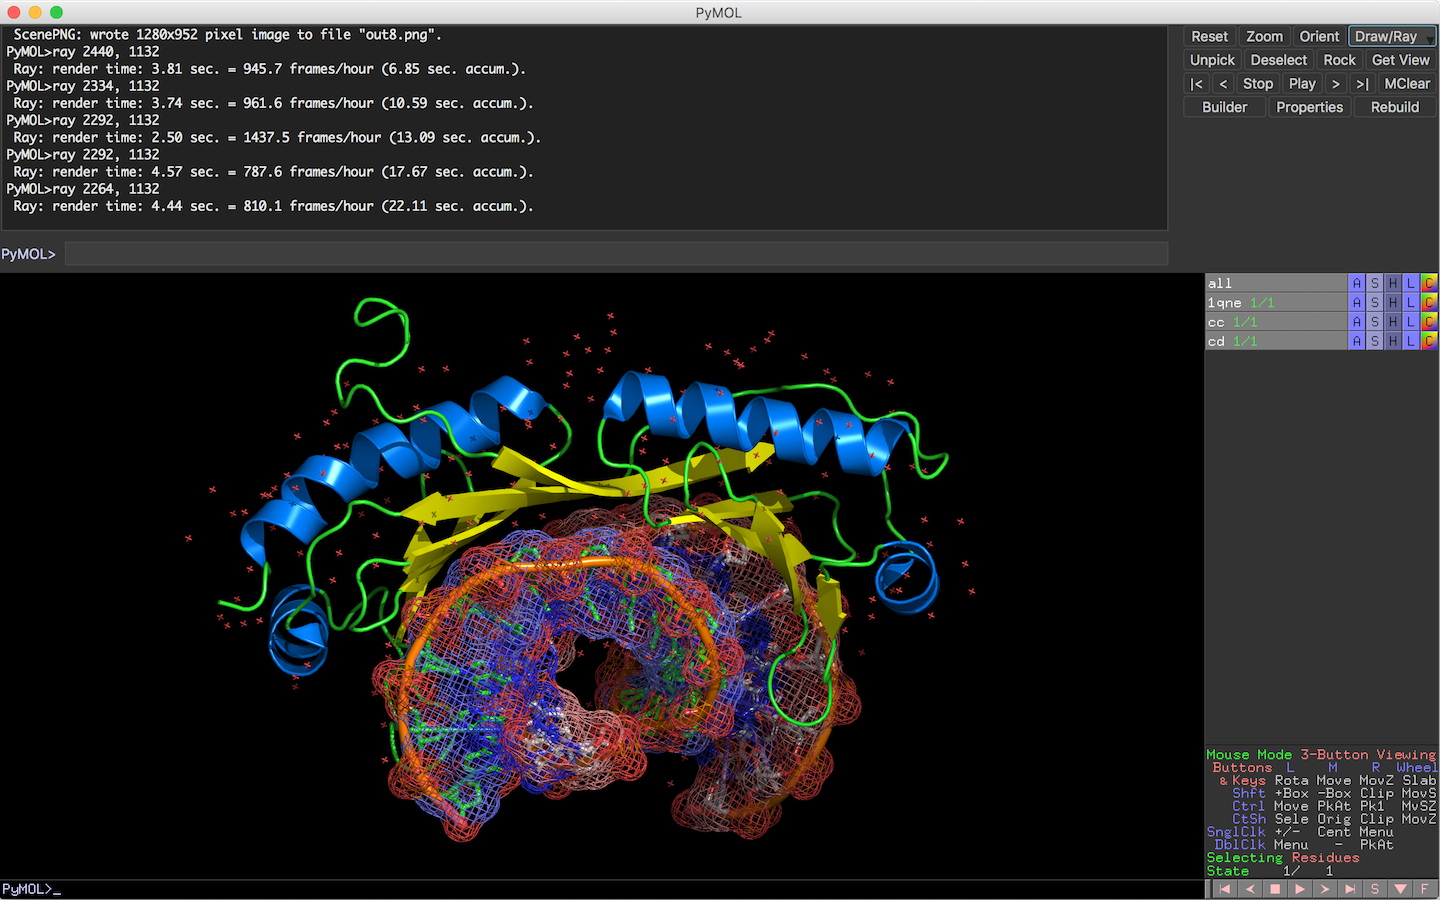
\includegraphics[scale=0.47]{../pictures/pic3.png}
\end{frame}

\section{Алгоритм выравнивания}
\begin{frame}
\frametitle{Структурное выравнивание}
\begin{center}
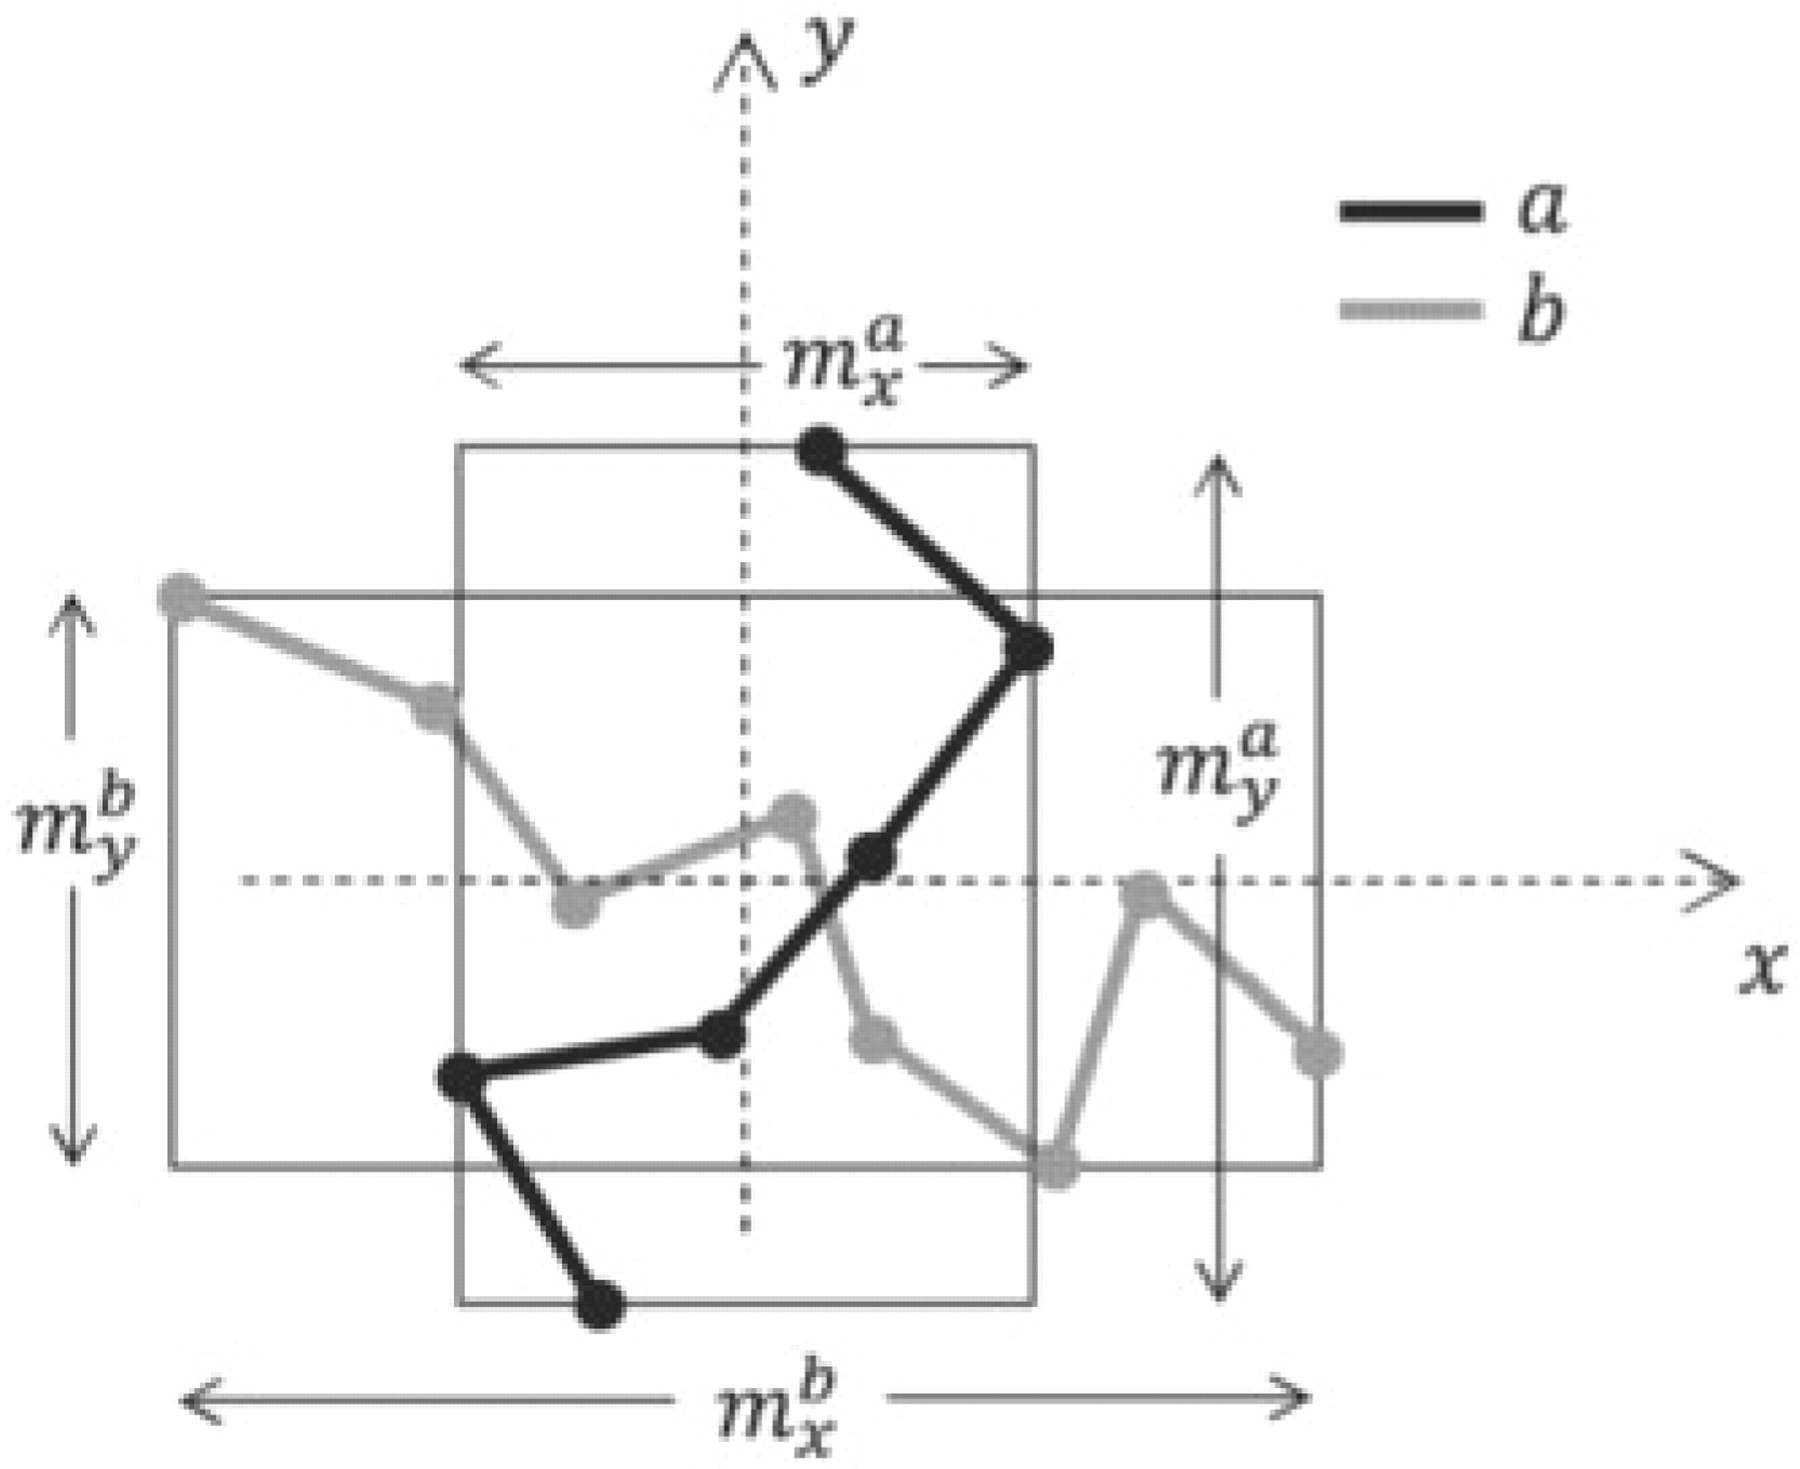
\includegraphics[scale=0.15]{../pictures/btp530f1.jpeg}
\end{center}
\end{frame}

\begin{frame}
\frametitle{Метрики качества}
\begin{itemize}
\item $CA \leq \sigma$
\pause
\vfill
\item GDT\_TS
\pause
\vfill
\item ALo
\pause
\vfill
\item MaxSub
\pause
\vfill
\item TM-score
\pause
\vfill
\item Q-score
\end{itemize}
\end{frame}

\begin{frame}
\frametitle{Альфа-карбоны}
\begin{center}
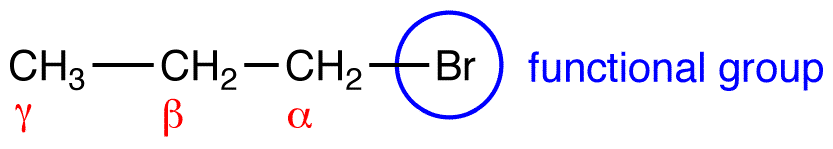
\includegraphics[scale=1.4]{../pictures/pic4.png}
\vfill
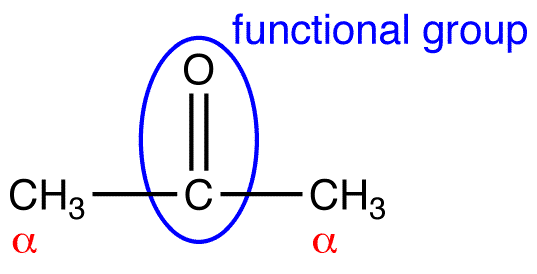
\includegraphics[scale=1.4]{../pictures/pic5.png}
\end{center}
\end{frame}

\begin{frame}
\frametitle{Пространство допустимых решений}
\begin{center}
\begin{gather*}
t = (\alpha, \beta, \gamma, u, v, w)\\
I = [0, 2\pi] \times [0, \pi] \times [0, 2\pi] \times [-M_x, m_x] \times [-M_y, M_y] \times [-M_z, M_z]\\
M_x = \frac{m_x^a + m_x^b}{2}\\
M_y = \frac{m_y^a + m_y^b}{2}\\
M_z = \frac{m_z^a + m_z^b}{2}\\
\end{gather*}
\end{center}
\end{frame}

\begin{frame}
\frametitle{$\eps$-сеть}
\begin{center}
\begin{gather*}
r_{\alpha, \gamma} =  \frac{6\sqrt{2}\pi R_b}{\eps}\\
r_{\beta} =  \frac{3\sqrt{2}\pi R_b}{\eps}\\
s_x = 1 + \frac{2\sqrt{3}M_x}{\eps}\\
s_y = 1 + \frac{2\sqrt{3}M_y}{\eps}\\
s_z = 1 + \frac{2\sqrt{3}M_z}{\eps}\\
d_r = \frac{\eps}{3\sqrt{2}R_b}\\
d_t = \frac{\eps}{\sqrt{3}}\\
\end{gather*}
\end{center}
\end{frame}

\begin{frame}
\frametitle{Временная сложность}
В $\eps$-сети находится $O(\frac{n^6}{\eps^6})$ ячеек.
\vfill
Для подсчёта результата метрики требуется $O(n^2)$ времени.
\vfill
Общая сложность алгоритма $O(\frac{n^8}{\eps^6})$.
\end{frame}

\begin{frame}
\frametitle{Поиск оптимального решения}
\begin{algorithmic}[1]
\State $\eps \la 1$
\State $t_\eps^\sigma \la \mathrm{EPSILON-OPTIMAL}(a, b, \sigma, \eps)$
\State $t_eps^{\sigma - \eps} \la \mathrm{EPSILON-OPTIMAL}(a, b, \sigma - \eps, \eps)$
\State $\eps \la \frac{\eps}{2}$
\While{$|S(a, t_\eps^\sigma (b), \sigma + \eps )| - |S(a, t_\eps^{\sigma - \eps}(b), \sigma ) > 0$}
\State $t_\eps^\sigma \la \mathrm{EPSILON-OPTIMAL}(a, b, \sigma, \eps)$
\State $t_eps^{\sigma - \eps} \la \mathrm{EPSILON-OPTIMAL}(a, b, \sigma - \eps, \eps)$
\State $\eps \la \frac{\eps}{2}$
\EndWhile
\State \Return $t_\eps^{\sigma - \eps}$
\end{algorithmic}
\end{frame}

\section{Результаты}

\begin{frame}
\frametitle{База данных Scope}
Набор для тестирования содержит 195 пар белков связанных на различных условиях согласно структурной классификации SCOP: 57 family пар, 75 superfamily пар, и 63 fold-пары.\\
\begin{table}[H]
\caption{ Общее число пар в тестовом наборе, которые могут быть наложены на расстояние не превосходящем 3 \angstrom}
\begin{center}
\begin{tabular}{|c|ccccc|}
\hline
& MAX-PAIRS & LGA & TM-alogn & Mammoth & Mustang\\
\hline
Family & 4689 & 4585 & 4460 & 4264 & 4231\\
Superfamily & 4378 & 4247 & 4140 & 3713 & 3319\\
Flod & 2870 & 2720 & 2634 & 2100 & 1834\\
\hline
\end{tabular}
\end{center}
\end{table}
\end{frame}

\begin{frame}
\frametitle{База данных Scope}
Набор для тестирования содержит 195 пар белков связанных на различных условиях согласно структурной классификации SCOP: 57 family пар, 75 superfamily пар, и 63 fold-пары.\\
\begin{table}[H]
\caption{ Общее число пар в тестовом наборе, которые могут быть наложены на расстояние не превосходящем 5 \angstrom}
\begin{center}
\begin{tabular}{|c|ccccc|}
\hline
& MAX-PAIRS & LGA & TM-alogn & Mammoth & Mustang\\
\hline
Family & 5261 & 5130 & 5059 & 5019 & 4983\\
Superfamily & 5240 & 5033 & 4928 & 4702 & 4532\\
Flod & 3575 & 3409 & 3279 & 2842 & 2816\\
\hline
\end{tabular}
\end{center}
\end{table}
\end{frame}
\end{document}